\documentclass[11pt,titlepage,dvipdfmx,twoside]{jarticle}
\linespread{1.1}

\usepackage{amsfonts}
\usepackage{amssymb}
\usepackage{amsmath}
\usepackage{amsthm}
\newtheorem{theorem}{Theorem}
\newtheorem{lemma}[theorem]{Lemma}
\usepackage{enumitem}
\usepackage{geometry}
\geometry{left=2.5cm,right=2.5cm,top=2.5cm,bottom=2.5cm}

\usepackage{algorithm}  
\usepackage{algorithmic}  
\renewcommand{\algorithmicrequire}{\textbf{Input:}} 
\renewcommand{\algorithmicensure}{\textbf{Output:}}
\renewcommand{\algorithmicforall}{\textbf{for each}}

\usepackage{mathtools}
\usepackage{comment}
\usepackage[dvipdfmx]{graphicx}
\usepackage{float}
\usepackage{framed}
\usepackage{graphicx}
\usepackage{subcaption}
\usepackage{listings}
\usepackage{plistings}
\usepackage{color}
\usepackage{url}

\definecolor{codegreen}{rgb}{0,0.6,0}
\definecolor{codegray}{rgb}{0.5,0.5,0.5}
\definecolor{codepurple}{rgb}{0.58,0,0.82}
\definecolor{backcolour}{rgb}{0.95,0.95,0.92}
 
\lstdefinestyle{mystyle}{
    %backgroundcolor=\color{backcolour},   
    frame=single,
    commentstyle=\color{codegreen},
    keywordstyle=\color{magenta},
    numberstyle=\tiny\color{codegray},
    stringstyle=\color{codepurple},
    basicstyle=\footnotesize,
    breakatwhitespace=false,         
    breaklines=true,                 
    captionpos=b,                    
    keepspaces=true,                 
    numbers=left,                    
    numbersep=5pt,                  
    showspaces=false,                
    showstringspaces=false,
    showtabs=false,                  
    tabsize=2
}
\renewcommand{\lstlistingname}{図}
\lstset{style=mystyle}

\title{\Huge{Pythonのscikit-learnを用いたニューラルネットワーク
による学習とデータ取得方法}}

\begin{document}

% The following makeatletter must be after begin{document}
\makeatletter 
\let\c@lstlisting\c@figure
\makeatother

\西暦
\date{\today}

\maketitle

% \cleardoublepage

\thispagestyle{empty}
\tableofcontents
\clearpage

\pagenumbering{arabic}

\section{概要}
この冊子では,化合物の既知のデータと性質を与えられて,未知の化合物の特性を予測する人工ニューラルネットワークを構築する方法を説明する.
そのために,化合物は化合物の構造から得られた特徴ベクトルとして表される.
化合物の特徴ベクトルといくつかの化学的性質を表す値の組を与えられるプログラムを説明し,人工ニューラルネットワークを構築し,訓練済みニューラルネットワークのパラメータ(重みとバイアス)を取得する方法を説明する.

プログラミング言語Pythonでの機械学習にはscikit-learnライブラリを使用する.

次のWebページで詳細を確認してください

https://scikit-learn.org/stable/

この冊子には次の3つのファイルを伴うことに注意してください.

\begin{itemize}
\item {\tt scikit\_chemgraph\_learning.py}\\
Pythonで記述されたプログラムで,特徴ベクトルと化学的性質の観測値の組のデータセットを与え,5分割交差検証を用いて人工ニューラルネットワークを構築する.
テストデータに対して最も高い決定係数(${\rm R}^2$)スコアを実現する訓練済みニューラルネットワークの重みとバイアスは,出力ファイルとして保存される.
詳細は第\ref{sec:section4}節を参照すること.

\item {\tt ha\_fv4\_plus.csv} \\
PubChemデータベースにある特性「霧化熱」の既知の値を持つ化合物の計算済み特徴ベクトル.

\item {\tt ha\_target\_data.csv}\\
PubChemデータベースにある化合物の特性「霧化熱」の観測値のカンマ区切り値ファイルである.

 \medskip 
第\ref{sec:section3}節にはファイル形式の詳細が含まれ、第\ref{sec:section5}節には上記の2つのファイルのデータセットを使用した計算実験の結果を示す。
\end{itemize}

次に,この冊子の構成について説明する.
第\ref{sec:section2}節では,この冊子およびプログラム内
で使用している基本的な用語について説明する.
第\ref{sec:section3}節では,プログラムの入力と出力の形式について説明する.特にプログラムの入出力の実際の例が使用されている.
第\ref{sec:section4}節では,プログラムのソースコードの詳細を示す.
実際のソースコード内での操作について説明する.
第\ref{sec:section5}節では,実際の計算実験の結果を示す.
\newpage

\section{用語の説明}
\label{sec:section2}
この節では,冊子の本文中で使用する用語について説明する.

\begin{itemize}
\item 特徴ベクトル\\
各元素の種類の原子数等の化学物質を説明する数値,あるいはグラフの直径等の化学物質のグラフ表現のトポロジーに基づいて計算される数値のベクトル
\item ニューラルネットワーク \\
人工ニューラルネットワーク,または単にニューラルネットワークとは,機械学習で最も確立した手法の1つである.これらは入力ベクトルに基づいて値を予測するために用いられる.この冊子では,ニューラルネットワークへの入力は,化合物の特徴ベクトルであり,出力は特定の化学的性質の予測値である.
\item 入力層,隠れ層,出力層\\
人工ニューラルネットワークの多層パーセプトロンモデルを仮定する.このモデルでは,ニューラルネットワークはいくつかの層で構成されている.最初の層は入力層で,入力層は場合によっては特徴ベクトルから数値データを得るため,特徴ベクトルの要素と同じ数のノードがある.次に数値は隠れ層を介して伝播される.隠れ層は1つの層の計算が次の層への入力として用いられる.最後に出力層が入力ベクトルに基づいた予測値を与える.
\item ウェイト\\
ニューラルネットワークに含まれているノード間を接続している枝はそれぞれ値を持っており,その値をウェイトと呼ぶ.入力層から出力層への値の伝播には,これらのウェイトに基づく計算が含まれている.

\item バイアス\\
ニューラルネットワークの隠れ層の各ノードにはバイアスと呼ばれる数値が割り当てられている.この数値はウェイトと共に,入力ベクトルに基づいて出力値を計算する過程で使用される.
\medskip

ニューラルネットワークは与えられた入力ベクトルと目標値の組に基づいてウェイトとバイアスの組を計算することで「学習」する.

\item 活性化関数\\
活性化関数はニューラルネットワークの各ノードに割り当てられており,与えられた入力ベクトルから出力値を計算する際に用いられる.特に各ノードの出力値は,重み付けされた対応する枝のウェイトと前の層からのノードの出力の線形結合を入力として与えられた活性化関数の値である.

\end{itemize}

\newpage

\section{プログラムの入力と出力}
\label{sec:section3}

この節では,Pythonプログラムの入力と出力の形式の詳細について説明する.
\ref{sec:section3_1}節では,
霧化熱の化学的性質を用いた実際の例を使ってプログラムの入力について説明する.
\ref{sec:section3_2}節では,
入力データの形式の詳細を説明する.
\ref{sec:section3_3}節では,
入力データから生成された出力について具体例を用いて説明する.
\ref{sec:section3_4}節では,
出力データの形式を説明する.

\subsection{プログラムの入力}
\label{sec:section3_1}

入力としてプログラムはデータファイルを2つ必要とする.1つは一連の化合物の特徴ベクトルのデータのファイルで,もう1つは同じ化合物のセットで,観測されたいくつかの化学的性質の数値データのファイルである.プログラムはこれらの2つのファイルを与えられると,ニューラルネットワークを構築及び訓練する.

\bigskip

\subsection{入力データの形式}
\label{sec:section3_2}

この節では,\ref{sec:section3_1}節で説明しているプログラムに入力する2つのファイルの形式について説明する.
まず特徴ベクトルが記述されているファイルの形式について説明する.これはプレーンテキスト形式のカンマ区切り値(csv)ファイルである.
最初の行は特徴ベクトルの各記述子の名前を示しており,最初の項目である化合物識別番号(CID)は学習や予測に使用されていない.
次に,2行目以降に化合物の特徴ベクトルが示されており,各値はカンマで区切られ,各特徴ベクトルは1列で示されている.

\bigskip

\begin{oframed}
{\bf 特徴ベクトルのデータ形式}(注:\verb|\\|は実際に改行しないことを示す.)\\\\
%\bigskip\bigskip
CID,n,M,C\_in,C\_ex,O\_in,O\_ex,S\_in,S\_ex,H,C1O\_in,C1O\_ex,C1C\_in,C1C\_ex,C2C\_in,C2C\_ex,\verb|\\| \\
C1S\_in,C1S\_ex,\ldots \\
263,5,128,1,3,0,1,0,0,10,0,1,0,3,0,0,0,0, \ldots \\
6560,5,128,2,2,0,1,0,0,10,0,1,1,2,0,0,0,0, \ldots \\
6568,5,128,2,2,0,1,0,0,10,0,1,1,2,0,0,0,0, \ldots \\
6386,5,128,1,3,0,1,0,0,10,0,1,0,3,0,0,0,0, \ldots \\
6276,6,126.667,2,3,0,1,0,0,12,0,1,1,3,0,0,0,0,\ldots \\
\hspace{5mm}\vdots
\\
\hspace{5mm}\vdots

\end{oframed}

次に,化学的性質の目標値を含んだcsvファイルの構造について説明する.
最初の行は単に「CID,a」と記述しており,CIDは化合物のID番号,aは目標値を示している.
次の行は特徴ベクトルのcsvファイルと同じ順序で,化合物のIDと目標値である.

\bigskip

\begin{oframed}
{\bf Target data file format (example of heat of atomization)}\\\\
%\bigskip\bigskip
CID,a \\
263,1329.95 \\
6560,1332 \\
6568,1334.14 \\
6386,1338.88 \\
6276,1609.92 \\
\hspace{5mm}\vdots
\\
\hspace{5mm}\vdots

\end{oframed}


\subsection{プログラムの出力}
\label{sec:section3_3}

このプログラムで出力される訓練後のニューラルネットワークの
具体例が図~\ref{fig:sample}である.
図\ref{fig:sample}は計算された枝のウェイトとノードのバイアスを用いて,訓練済みニューラルネットワークの例を示している.
プログラムの最終出力は,訓練済みニューラルネットワークのウェイトとバイアスをテキストファイルで出力する.

\begin{figure}[H]
  \centering
  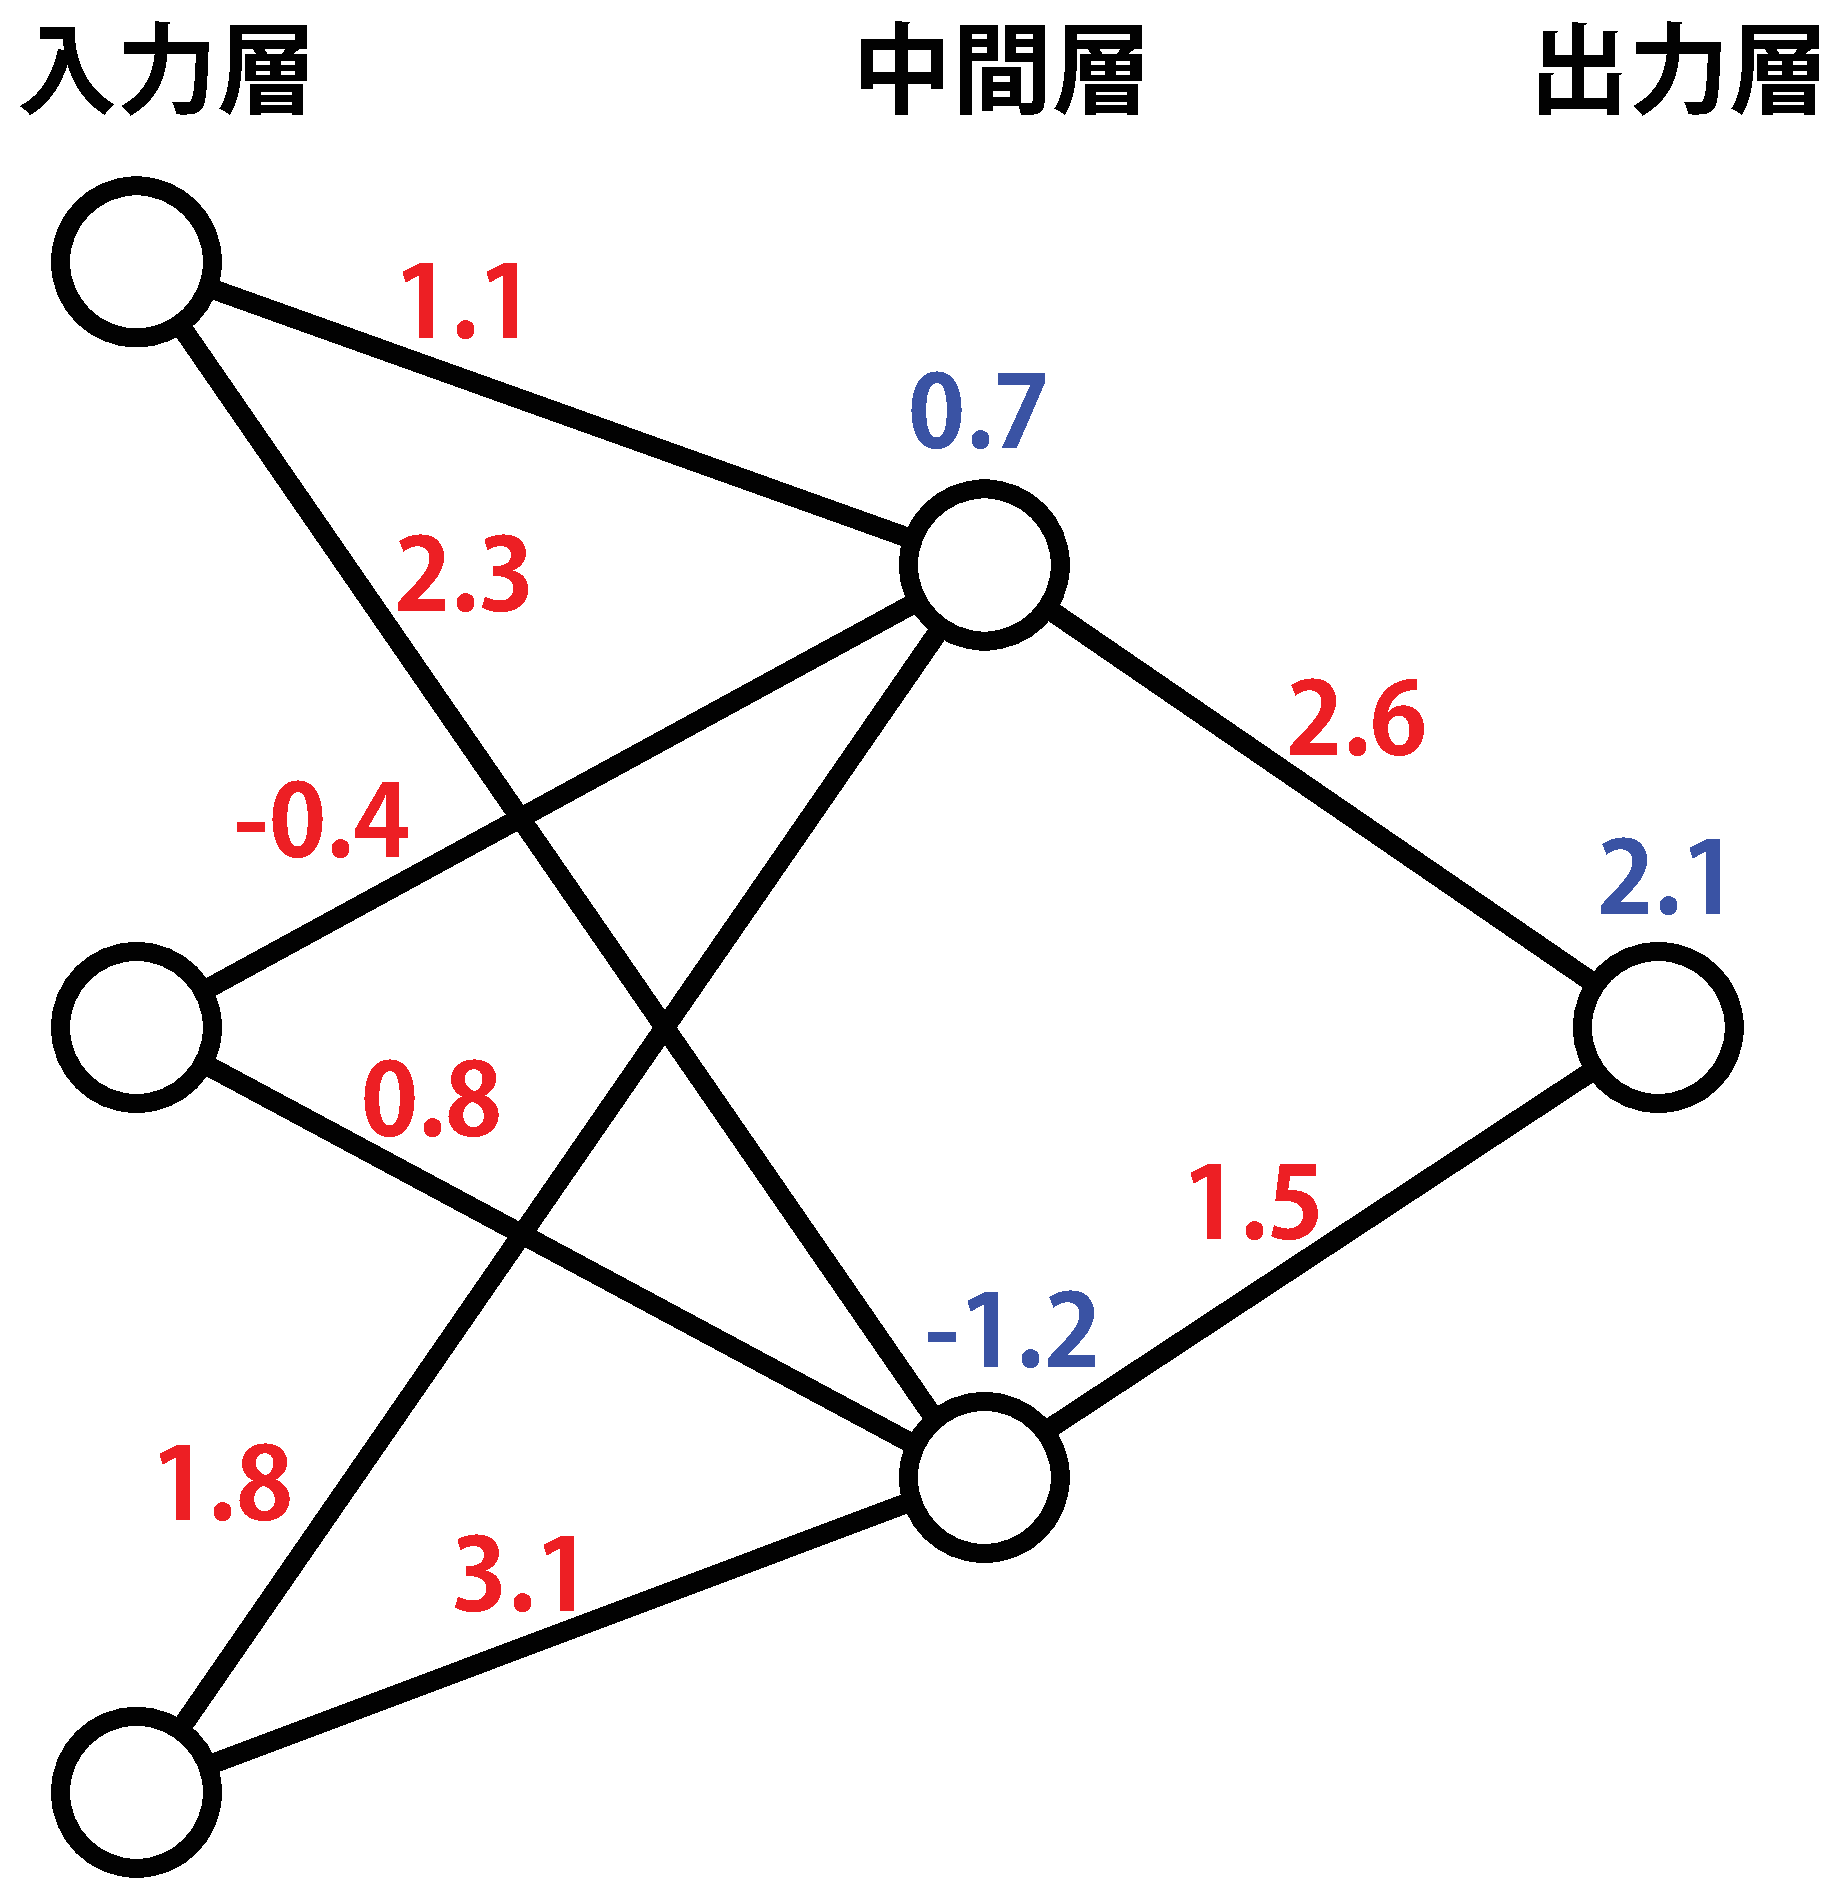
\includegraphics[width = 0.4 \textwidth]{./fig/ANN_sample_jp}
  \caption{学習後のニューラルネットワークの具体例.
  赤色の数値がウェイト,青色の数値がバイアスを表している.}
  \label{fig:sample}
\end{figure}


\subsection{出力データの形式}
\label{sec:section3_4}

訓練済みニューラルネットワークから生じる枝のウェイトとノードのバイアスはそれぞれ2つの出力ファイルに書き込まれる.

枝のウェイトのデータの出力ファイルの最初の行は人口ニューラルネットワークの構造,つまり入力層のノード数,各隠れ層のノード数,最後に出力層のノード数である.2行目以降は枝のウェイトの値である.各行は1つのノードから出る枝のウェイトの値を示す.

\bigskip

\begin{oframed}
{\bf ウェイトのデータ形式}\\\\
%\bigskip\bigskip
3 2 1\\
1.1 2.3\\
-0.4 0.8\\
1.8 3.1\\
2.6\\
1.5\\
\end{oframed}

\bigskip

ノードのバイアスを含むファイルには1行につき1つのノードのバイアスの値が示されている.入力層のノードにはバイアスの値がないことに注意.

\bigskip

\begin{oframed}
{\bf バイアスのデータ形式}\\\\
%\bigskip\bigskip
0.7\\
-1.2\\
2.1\\
\end{oframed}

\bigskip

\newpage

\section{プログラムの説明}
\label{sec:section4}

この節では,第\ref{sec:section3_1}節と第\ref{sec:section3_2}節で説明した特徴ベクトルと目標値のデータの入力ファイルを読み取り,5分割交差検証を用いて人工ニューラルネットワークを訓練し,5つの交差検証テストで最も高い決定係数 (R$^2$)を実現するニューラルネットワークの枝のウェイトとノードのバイアスのデータの出力ファイルを生成するプログラムについて説明する.出力ファイルの形式は第\ref{sec:section3_3}節と第\ref{sec:section3_4}節で説明している.プログラムのソースコードのファイル名は {\tt scikit\_chemgraph\_learning.py}としており,図\ref{code:ANN}に示す.

\bigskip\bigskip

\begin{lstlisting}[ language=Python,label={code:ANN},
  caption={ソースコードファイル{\tt scikit\_chemgraph\_learning.py}.},
  firstnumber = 3,]
"""
scikit_chemgraph_learning.py

This file implements functions that given a file with
descriptor values of chemical compounds and a file with target values,
performs 5-fold learning using an artificial neural network (MLP regressor)
and stores the weights and biases of the training iteration that achieved
the highest R^2 test score over the 5 trials. 

Command line arguments include
 - filename with a list of descriptors
 - filename with a list of target values
 - filename for the output weights and biases
 - network architecture, as a list of hidden layer sizes
 
The program will output on the terminal the R^2 and MAE scores, and
time taken for training for each 
trial in the 5-fold cross-validation, 
and the averages over the 5 trials at the end.
"""

import numpy as np
import pandas as pd
from sklearn.model_selection import KFold
from sklearn.neural_network import MLPRegressor
from sklearn.metrics import mean_absolute_error
import time
import sys

def write_weights_biases(reg, filename):
    """ 
    This function will write to disk 2 files, called
        "filename_weights.txt" and
        "filename_biases.txt"
    containing the weights and biases 
    of a trained artificial neural network reg given as an argument
    """
    # initialize separate filenames
    weights_filename = filename + "_weights.txt"
    biases_filename = filename + "_biases.txt"
    
    # Get the weights and biases from the trained MLP regressor
    weights = reg.coefs_
    biases = reg.intercepts_
    num_features = weights[0].shape[0]
    
    # Write the weights to file weights_filename
    with open(weights_filename, 'w') as f:
        f.write(str(num_features) + ' ')
        for i in range(len(reg.hidden_layer_sizes)):
            f.write(str(reg.hidden_layer_sizes[i]) + ' ')
        f.write('1\n')
        for item in weights:
            for i in range(item.shape[0]):
                for j in range(item.shape[1]):
                    if abs(item[i][j]) > 10**(-308):
                        f.write(str(item[i][j]) + ' ')
                    else:
                        f.write('0 ')
                f.write('\n')
    
    # Write the biases to a file biases_filename
    with open(biases_filename, 'w') as f:
        for item in biases:
            for i in range(item.shape[0]):
                f.write(str(item[i])+ '\n')
    

def train_ANN(descriptors_filename, target_values_filename, architecture):
    """
    Given filenames of a file containing a list of descriptors
    and a file containing target values, and a tuple of integers
    giving the number of nodes in hidden layers of an ANN,
    perform 5-fold cross-validation learning by using the 
    descriptors and target values with an ANN of the given architectire,
    and return the trained ANN (MLP regressor) that achieved the highest
    R^2 test score over the test data.
    """
    
    # read the training and target data
    fv = pd.read_csv(descriptors_filename) 
    value = pd.read_csv(target_values_filename)       
    
    # prepare target, train, test arrays
    target = np.array(value['a'])
    
    x = fv.values[:,1:]
    y = target
    
    print('n range = [{},{}]'.format(fv['n'].min(),fv['n'].max()))
    print('a range = [{},{}]'.format(value['a'].min(),value['a'].max()))
    
    numdata = x.shape[0]
    numfeature = x.shape[1]
    print('#instances = {}'.format(numdata))
    print('#features = {}'.format(numfeature))
    
    # Initialize an artificial neural network - MLP regressor
    reg = MLPRegressor(activation='relu', solver='adam',
                       alpha=1e-5, hidden_layer_sizes=architecture,
                       random_state=1, max_iter=100000000)
    
    score_R2 = np.array([])
    score_MAE = np.array([])
    time_train = np.array([])
    
    # Separate the data randomly for cross-validation
    kf = KFold(n_splits=5, shuffle=True, random_state=21)
    fold = 0
    for train, test in kf.split(x):
        fold += 1
        x_train, x_test, y_train, y_test = x[train], x[test], y[train], y[test]
        print('\nD{}: train {}, test {}'.format(fold, 
              x_train.shape[0], x_test.shape[0]))
    
        start = time.time()
        reg.fit(x_train, y_train)
        end = time.time()
        timetemp = end-start
        
        print('training time: {}'.format(timetemp))
        time_train = np.append(time_train, timetemp)
    
        pred = reg.predict(x)
        pred_train = reg.predict(x_train)
        pred_test = reg.predict(x_test)
           
        # calculate the prediction score (R^2)
        R2train = reg.score(x_train,y_train)
        R2test = reg.score(x_test,y_test)
        R2all = reg.score(x,y) 
        print('R2 score train = {}'.format(R2train))
        print('R2 score test = {}'.format(R2test))
        print('R2 score all = {}'.format(R2all))
        temp = np.array([R2train, R2test, R2all]).reshape(1,3)
        score_R2 = np.append(score_R2, temp)
        
        # check the test R2 score and store the regressor with the highest one
        if (fold == 1):
            best_regressor = reg
            best_R2_score = R2test
        else:
            if (R2test > best_R2_score):
                best_regressor = reg
                best_R2_score = R2test

    score_R2 = score_R2.reshape(5,3)
    avg_time = np.mean(time_train)
    print('\nAverage time = {}'.format(avg_time))
    avg_testR2 = np.mean(score_R2, 0)[1]
    print('Average R2 test score = {}'.format(avg_testR2))
    
    return best_regressor


def main(argv):
    if (len(argv) < 5):
        print("""
              Please supply at least 4 command line arguments:
                  - Descriptors as training data
                  - Target values as training data
                  - Filename for the output weights/biases files
                  - number of nodes in at least one hidden layer
                  
              The program will now terminate.""")
        sys.exit()
    # else:
    # Parse the command line arguments
    descriptors_filename = argv[1]
    target_values_filename = argv[2]
    output_filename = argv[3]
    architecture = tuple(int(a) for a in argv[4:])
    
    # Perform 5-fold validation with the given training data
    # and return the regressor that achieves highest R^2 test score
    best_regressor = train_ANN(descriptors_filename,
                                               target_values_filename,
                                               architecture)
    
    # Write the weights and biases of the regressor to files
    write_weights_biases(best_regressor, output_filename)
    
    
main(sys.argv)
\end{lstlisting}

プログラムは,活性化関数としてRectified Linear Unit function(ReLU関数)を用いて101行目で人工ニューラルネットワークを初期化している.
人工ニューラルネットワークのハイパーパラメータの詳細は以下に添付している公式のscikitウェブページで確認してください.
\\

\url{https://scikit-learn.org/}

% https://scikit-learn.org/stable/modules/generated/sklearn.neural\_network.MLPRegressor.html



\newpage

\section{プログラムの実行と計算例}
\label{sec:section5}

この節ではプログラムの実行例を使用してプログラムの実行方法を説明する.
霧化熱の目標値のデータとPubChemデータベースから取得した化合物の特徴ベクトルを訓練データとして使用する.

\subsection{実行方法}
\label{sec:section5_1}

Python3を実行できる環境であることを確認してください.必要な付属パッケージが多く含まれているAnaconda等のディストリビューションを使用することを推奨する.
\\
\url{https://www.anaconda.com/distribution/}

プログラムのソースコードである\verb|scikit_chemgraph_learning.py|とその入力ファイルである\verb|ha_fv4_plus.csv|と \verb|ha_target_data.csv|は同じフォルダにあると仮定する.
例として,10個のノードを持つ1つの隠れ層をアーキテクチャとして人工ニューラルネットワークを構築する.
人工ニューラルネットワークの結果として枝のウェイトとノードのバイアスは\verb|ANN_weights.txt|と\verb|ANN_biases.txt|にそれぞれ書き込まれる.

コードを実行するにはPythonが有効になっているターミナルで次のように入力する.
\begin{verbatim}
 python3 scikit_chemgraph_learning.py ha_fv4_plus.csv ha_target_data.csv ANN 10
\end{verbatim}

新しい2つのファイルである\verb|ANN_weights.txt|と\verb|ANN_biases.txt|がフォルダに作成され,それぞれ枝のウェイトとノードのバイアスが記述されるはずである.
計算中にプログラムは訓練データのサンプル数,ネットワークの訓練にかかった時間, R$^2$スコアを含んだ各交差検証の試行毎の状況をターミナルに出力する.


\subsection{計算例}
\label{sec:section5_2}

ここではサンプル入力ファイルの\verb|ha_fv4_plus.csv |と\verb|ha_target_data.csv|を用いてプログラムを実行して得られた結果を示す.

まず,訓練済み人工ニューラルネットワークの枝のウェイトの出力ファイル\verb|ANN_weights.txt|の内容を示す.ファイル形式は第\ref{sec:section3_4}節で説明している.

\bigskip

\begin{oframed}
{\bf ANN\_weights.txtの具体例(原子化熱の場合)}\\\\
22 10 1  \\
-1.1238112931499422e-84 3.0170452635900533 -1.6241043622384792e-73 -3.6018735325629394 -8.391988020519093e-77 2.3580716556323953 -0.026736972121934502 2.575726292584817 -2.063731712717064e-06 4.597303330113335   \\
-9.344488035266295e-85 1.497290480000622 -3.036274715861717e-78 1.8156784526785696 -4.3151757452976e-74 1.4217041980099014 -0.023459434269884616 1.3379213810845205 -0.011238853071123057 -0.7443192517629607   \\
4.132475087678266e-78 3.3990565079553554 -2.868320003068728e-81 -3.4651919683025674 2.9940970334531404e-76 3.2165216940835757 -0.03213106633429949 2.472993257729317 -2.1917950390948578e-06 4.771137374239634   \\
-1.1581526717811436e-75 -1.329707686671036 2.0796776718616044e-74 6.237593937811961 4.1273697169652248e-81 -1.4062510180009142 -0.026704728711823528 -0.925294417115918 -6.740518660092261e-74 -5.540003285685092   \\
9.543615511411743e-74 -1.1589876575808225 -2.6364157708348452e-80 3.187561980333966 -8.943738918434615e-76 -1.4524340822049775 0.051782929796906886 -1.5653228064901121 -1.6249155288107357e-80 -3.634647585954396   \\
-6.39468464326263e-74 3.0629683725323584 -1.9774305352016877e-78 -3.7172015955219266 -3.7919200519635786e-88 2.4044443070857207 -0.02401369830407232 2.4832637050782376 -0.00022794649906475431 4.66431434861339   \\
-9.377192677863584e-76 3.004803749408999 4.902837933366572e-81 -2.5013050438170104 -1.4036823325175825e-74 2.998787164164196 -0.026861635340365342 2.981392380037406 1.0661485018096706e-74 2.3304790128834076   \\
1.2701574125840252e-75 2.7221295483347125 -1.2703118087438868e-76 -2.9194172521756747 -5.544716411580953e-84 2.630411509774059 -0.015116670855903482 2.7865193029822377 -8.887535520464753e-07 4.436851466042201   \\
4.351938047328309e-76 1.1180131069815742 1.9824013505096927e-79 0.9464827643663908 -5.2330770435602964e-80 1.2998557027642679 -0.0271136889312177 1.3721987711511763 5.654281723895746e-82 -1.1521340765967187   \\
-4.832882183847715e-76 -0.984636501818488 -5.8925978392141506e-86 3.0049263389599625 -2.3626537886806268e-84 -1.6350496714029827 0.05142288752338433 -1.3227793558667296 -1.422705004455725e-73 -3.6206407833583314   \\
-1.1423162173298355e-81 2.5902312579960958 5.014920153233757e-76 -3.4344337828410194 1.6638832030159978e-75 2.5636947094464215 -0.03842125857490203 2.8294384537406594 -3.378684191548278e-07 4.509451556355702   \\
-1.9791643476720933e-77 2.575887805003329 5.789281131361252e-75 -2.7281627756446336 -6.220513272189593e-75 2.998889390482911 -0.022617802565271246 3.141560745624169 1.414233611426763e-19 4.20142249839257   \\
-6.236323873029463e-74 2.5328911726682506 -4.1242465272786166e-74 -4.325696725950309 1.2224358229010616e-76 2.8538143450705977 -0.027122334983233323 3.113071693728851 -2.904059652886194e-76 5.198706814683436   \\
1.420883684820555e-84 4.419013439859128 1.6389532350787483e-85 -4.979526814267058 4.1052218408326557e-78 3.652082980531675 -0.024619557800014336 3.7853797365655724 -3.116805665467011e-12 5.524734571674539   \\
1.0539941002876462e-85 -1.484006161426568e-76 -8.481259995666099e-75 -3.385627263079466e-76 -1.840734810369072e-74 -7.126209692448427e-76 -8.430081625400892e-79 1.7094068447294007e-80 1.4534199593339358e-85 -8.909642175302103e-74   \\
-4.579216934717519e-75 3.3160819289390773e-74 3.096517969737067e-85 -3.252893330112976e-78 -1.6131377874071942e-79 1.264042447674757e-79 -5.178853335658389e-78 9.79532619082707e-85 3.7975705026371116e-74 5.864667199962804e-77   \\
-3.527077784355358e-79 1.0055144424417832 2.2306081105728293e-83 1.3622446947832159 -4.785545338835612e-77 0.5400841311524589 -0.03624633129780699 0.9578106090827272 7.644113549863133e-84 -1.1524755436280696   \\
-2.1846619808211293e-81 9.430959196585263e-74 8.536075853537646e-85 -2.2139284118700775e-83 6.398633625096473e-86 1.3910501842751384e-79 8.538704976080743e-82 -7.228543198210997e-80 -6.114976978023107e-75 -4.7877245965779975e-83   \\
4.716163509148316e-83 1.3567662696569605 2.2217242689278444e-79 0.3595889984417734 -9.709418766252208e-80 1.7984676174734713 -0.026019205526194706 1.6645822669313806 -2.7524293292069654e-41 0.4640785972370295   \\
-8.022393348473078e-80 2.388617171015578 7.2218184954467e-80 -2.938485874134715 1.6022431880262786e-75 3.0259704996411654 -0.03858141275439007 2.420664143890053 -9.293345821386595e-11 4.428153114188145   \\
1.4128633719441486e-74 1.3504763123701526 2.4079461071148895e-75 2.836623998649334 -1.0226076926010233e-83 1.2329765686923553 -0.02707091168288496 1.2994911562472369 -2.684035828287667e-21 -0.9459205356006979   \\
-6.942528315035475e-84 1.5334486738127497 -1.804093649532225e-77 1.8778133808947834 -1.6006530414671997e-76 1.083156020823177 -0.04084555054335288 1.4765446070889678 -3.100280920791693e-21 0.11736440513790376   \\
-3.1879771652517114e-85   \\
1.916134889181373   \\
2.5464128802342342e-73   \\
-3.0910705862093906   \\
-1.444253829353331e-87   \\
2.0276392094212436   \\
-0.06469567595196621   \\
2.1390744407926197   \\
0.002829845412690173   \\
3.5091525125068657  \\
\end{oframed}

\bigskip

次に,訓練されたニューラルネットワークのノードのバイアスの出力ファイル\verb|ANN_biases.txt|の内容を示す.
ファイル形式については第~\ref{sec:section3_4}節を参照すること.

\bigskip

\begin{oframed}
{\bf ANN\_biases.txtの具体例}\\\\
-0.28042226851252594 \\
1.5596289736806637 \\
-0.31956610647035755 \\
-0.0872512930439685 \\
-0.1344620030528743 \\
2.008407301702276 \\
0.047331275321582 \\
1.9639995776527803 \\
0.27090672942420446 \\
1.6755999282930374 \\
0.7785606509372179
\end{oframed}

\bigskip

\begin{oframed}
{\bf  ターミナル画面に記述されたプログラムの出力}\\
\begin{verbatim}
n range = [4,11]
a range = [1100.6,3009.57]
#instances = 115
#features = 22

D1: train 92, test 23
training time: 5.539255857467651
R2 score train = 0.999972246284607
R2 score test = 0.9995125971676746
R2 score all = 0.9998742854857515

D2: train 92, test 23
training time: 5.087205410003662
R2 score train = 0.9998472762457117
R2 score test = 0.999827361127545
R2 score all = 0.9998423496039506

D3: train 92, test 23
training time: 5.4368956089019775
R2 score train = 0.9998628977117406
R2 score test = 0.9999531906631327
R2 score all = 0.999878508348101

D4: train 92, test 23
training time: 5.512180805206299
R2 score train = 0.999865105990373
R2 score test = 0.9999472183270992
R2 score all = 0.999877833093491

D5: train 92, test 23
training time: 6.058949947357178
R2 score train = 0.9998589982852477
R2 score test = 0.9999391731973049
R2 score all = 0.999876634586547

Average time = 5.526897525787353
Average R2 test score = 0.9998359080965512
\end{verbatim}
\end{oframed}

\bigskip\bigskip


%\newpage

%\begin{thebibliography}{99}
%  \bibitem{} 
%  \bibitem{} 
%  \bibitem{} 
%  \bibitem{} 
%\end{thebibliography}

\end{document}
